\section{Theory}

	\subsection{Electron Spin Resonance}

		Electron Spin Resonance can be understood from classical concepts. A particle having a magnetic moment $\mu$ is placed in a uniform magnetic field of intensity $H_0$, and the moment precesses about the field at a frequency called Larmor frequency is given by:

		$$\omega_0 = \frac{geH_0}{2mc}$$

		where g is the Lande g-factor ($g=1$ for pure orbital momentum and $g=2$ for a free electron spin). In the case of an ion in a crystal, the behaviour is modified by the environment and the g factor may differ from the Lande g-factor. This effective g-factor is known as the spectroscopic splitting factor.
		
		If now an additional weak magnetic field $H_1$ oriented in the x-y plane and rotating about the z axis (in the same direction as the ``Larmor processing'') with an angular frequency $\omega_1$ is introduced, there is a change in energy of the system.

		\begin{enumerate}
			\item For $\omega_1 \neq \omega_0$, the angle between the field $H_1$ and the magnetic moment $\mu$ will continuously change. Thus their average interaction will be zero.
			\item For $\omega_1 = \omega_0$, the angle between the field $H_1$ and the magnetic moment $\mu$ will be constant. Thus their net interaction is effective.
		\end{enumerate}

		This implies a change in the potential energy of the particle in the magnetic field. The change in $\theta$ is the classical analogy to a transition between sublevels with different $m$.

		Now considering the quantum picture, suppose the intrinsic angular momentum of the electron $S$ couples with the orbital angular momentum of electron $L$ to give a resultant $J$. We know, that $J+1$ magnetic sublevels are labelled by the magnetic field $H_0$ by equal energy difference. Now if we introduce a perturbation of the alternating magnetic field $H_1$ with a frequency corresponding to the energy difference between the levels $(h\nu)$, then there will be induced transitions between neighbouring sublevels according to the selection rules $\Delta m = \pm 1$ for magnetic dipolar radiation. Therefore, the condition for resonance is

		$$\Delta D = g\mu_0 H_0 = h\nu_0 = h\nu_1$$

		Where $\nu_1$ is the resonance frequency in cycles per second.

		\begin{figure}[H]
			\centering
			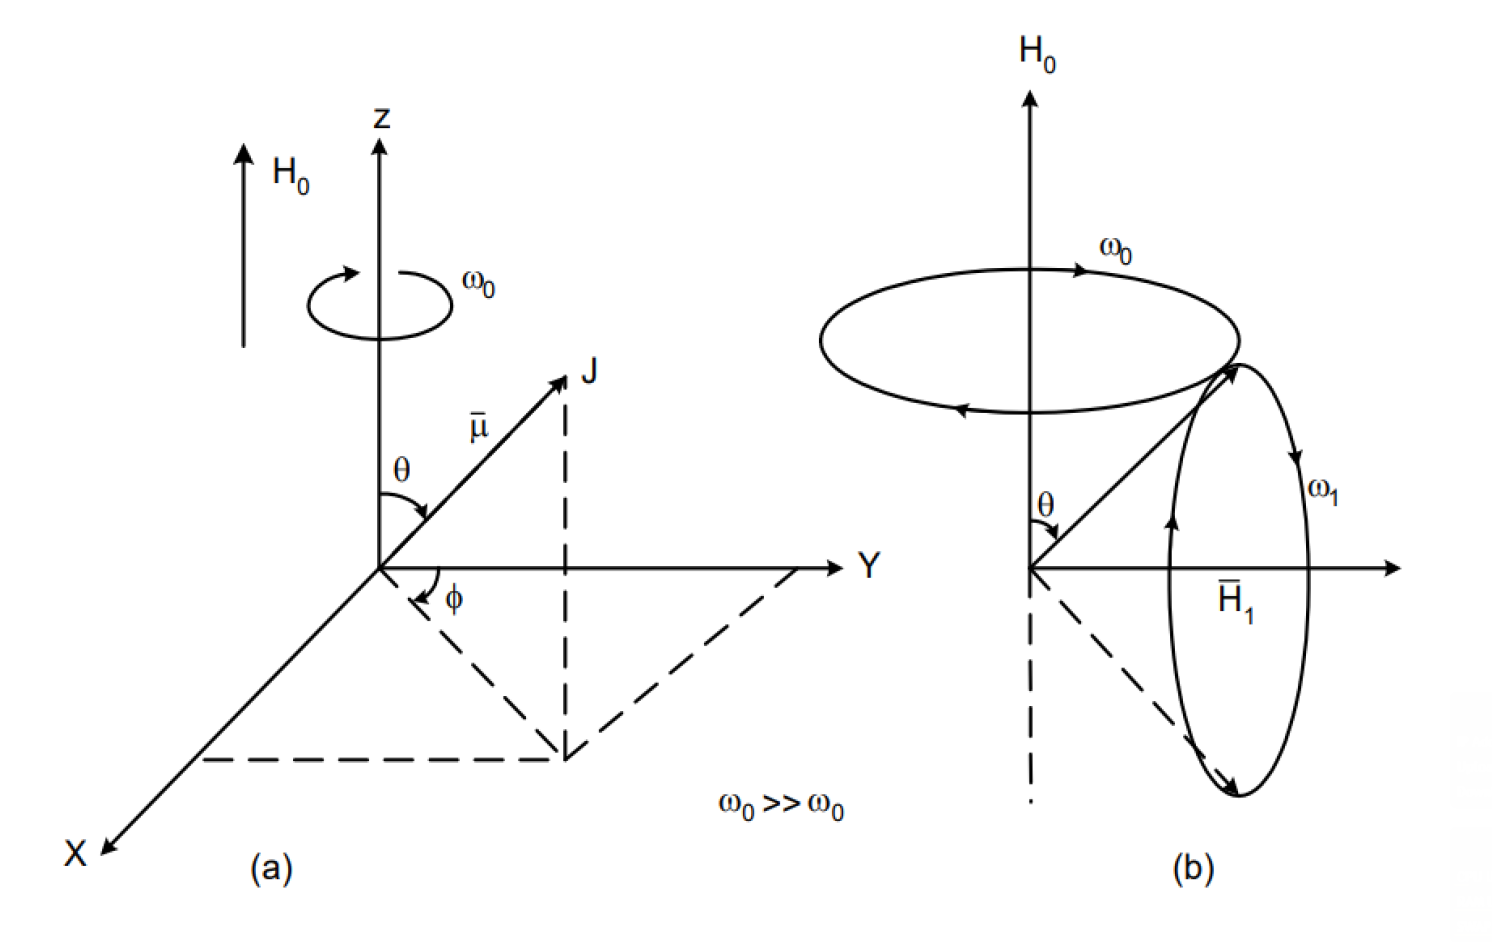
\includegraphics[width=0.5\textwidth]{magnetic_moment}
			\caption{\textbf{(a) Precession of a magnetic moment $\mu_1$ when placed in a magnetic field H0 where in (b) a weak field $H_1$ is applied.}}
			\label{fig:1}
		\end{figure}

	\subsection{Experimental Setup}
	
		The experimental setup consists of four parts:
		\begin{itemize}
			\item \textbf{Basic Circuit:} It consists of a critically adjusted(marginal) radio frequency oscillator having a frequency range of approximately 12-16MHz, which is required for the decrease in the amplitude of oscillation to an appreciable extent for the slightest increase in its load. There is a Helmholtz coil for the production of a magnetic field in and around the DPPH sample kept inside the tank coil. At resonance, an amplitude-modulated carrier is produced which is then detected using a diode detector and amplified by a chain of three low-noise, high-gain audio-frequency amplifiers (with sensitivity controls) of excellent stability.
				\begin{figure}[H]
					\centering
					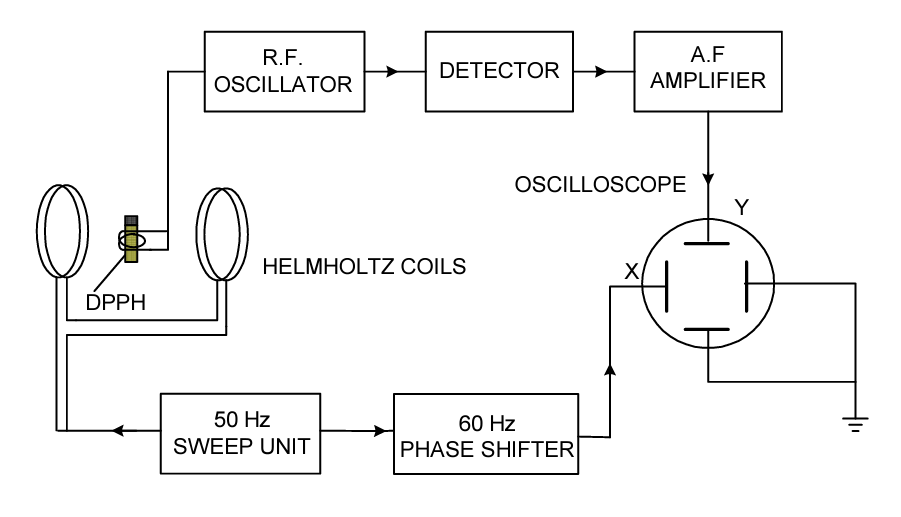
\includegraphics[width=0.5\textwidth]{ESR_Set.png}
					\caption{\textbf{Block diagram of ESR Circuit Setup}}
					\label{fig:2}
				\end{figure}
			\item \textbf{Phase Shifter:} To make it possible to use an ordinary displaying type oscilloscope, instead of a measuring oscilloscope which preserves the phase between X and plate signals, a phase shifter is provided. This can compensate for the phase difference which is introduced in the amplification stage of the ordinary oscilloscope as shown in \hyperref[fig:3]{Figure 3}.
				\begin{figure}[H]
					\centering
					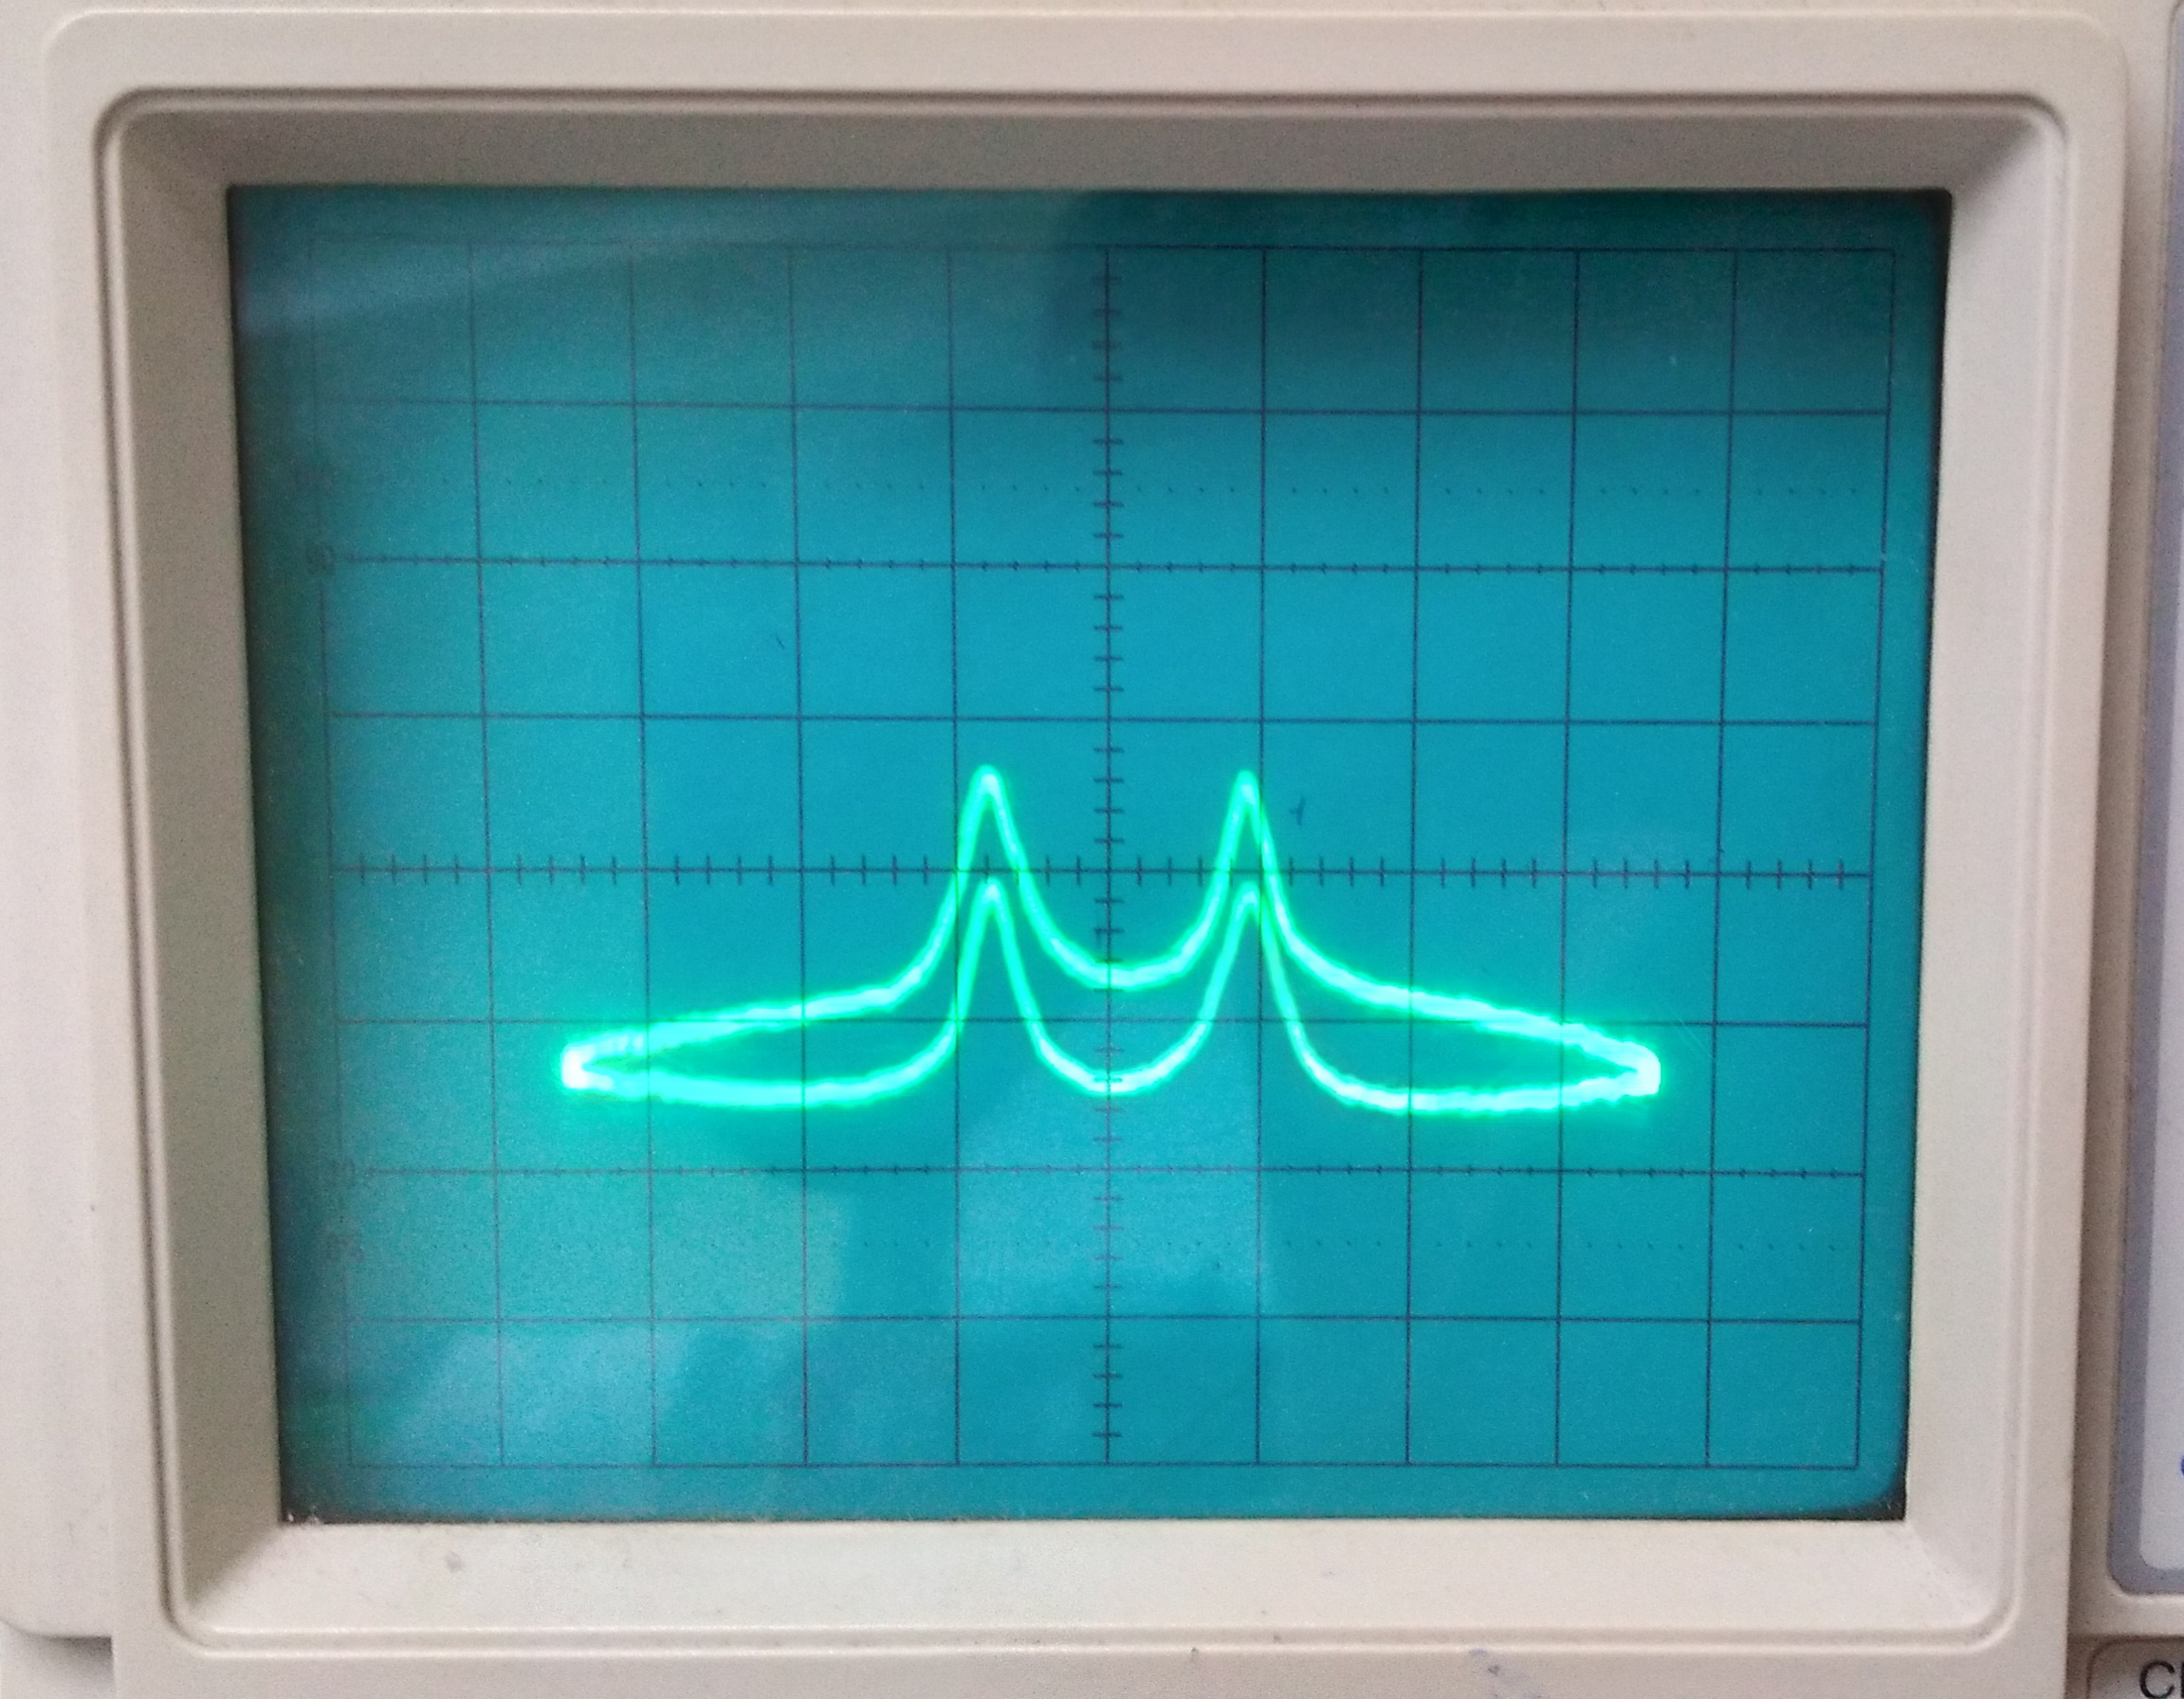
\includegraphics[width=0.4\textwidth]{photo.jpg}
					\caption{\textbf{Oscilloscope}}
					\label{fig:3}
				\end{figure}
			\item \textbf{50Hz Sweep Unit:} For modulation with a low-frequency magnetic field, a 50 Hz current flows through the Helmholtz coils.
			\item \textbf{Power Supplies:} DC Power supply for ESR circuit and the Helmholtz coils power supply consisting of a step-down transformer (220V to 35V AC).
			\item \textbf{Helmholtz Coil} of radius 7.5cm and 500 turns.
		\end{itemize}

	\subsection{Origin of Four Peaks}
		Observing the output in the oscilloscope, peaks can be found which are in fact absorption dips, because the sample absorbs power from the induction coil. The reason for getting peaks is due to an odd number of amplifying stages in the circuitry. The spin precesses with Larmor frequency $\omega_0$ vary in magnitude and direction due to variation of magnetic field H0 which is due to an alternating current in the Helmholtz coils. Now if the radio frequency field, $\omega_1 \approx \omega_0$ then resonance occurs. If the X plate signal (50Hz) and Y plate signal (ESR output) are in phase the I and II peaks and III and IV peaks will coincide. The coincidence of peaks on the x-scale needs to be calibrated for magnetic field measurements. The coincidence ensures that the magnetic field is zero at the centre and has peak values at the two ends. A complete merger of the peaks on the y-scale may not occur due to many reasons such as 50Hz pickups, ripples in the power supply etc.

		\begin{figure}[H]
			\centering
			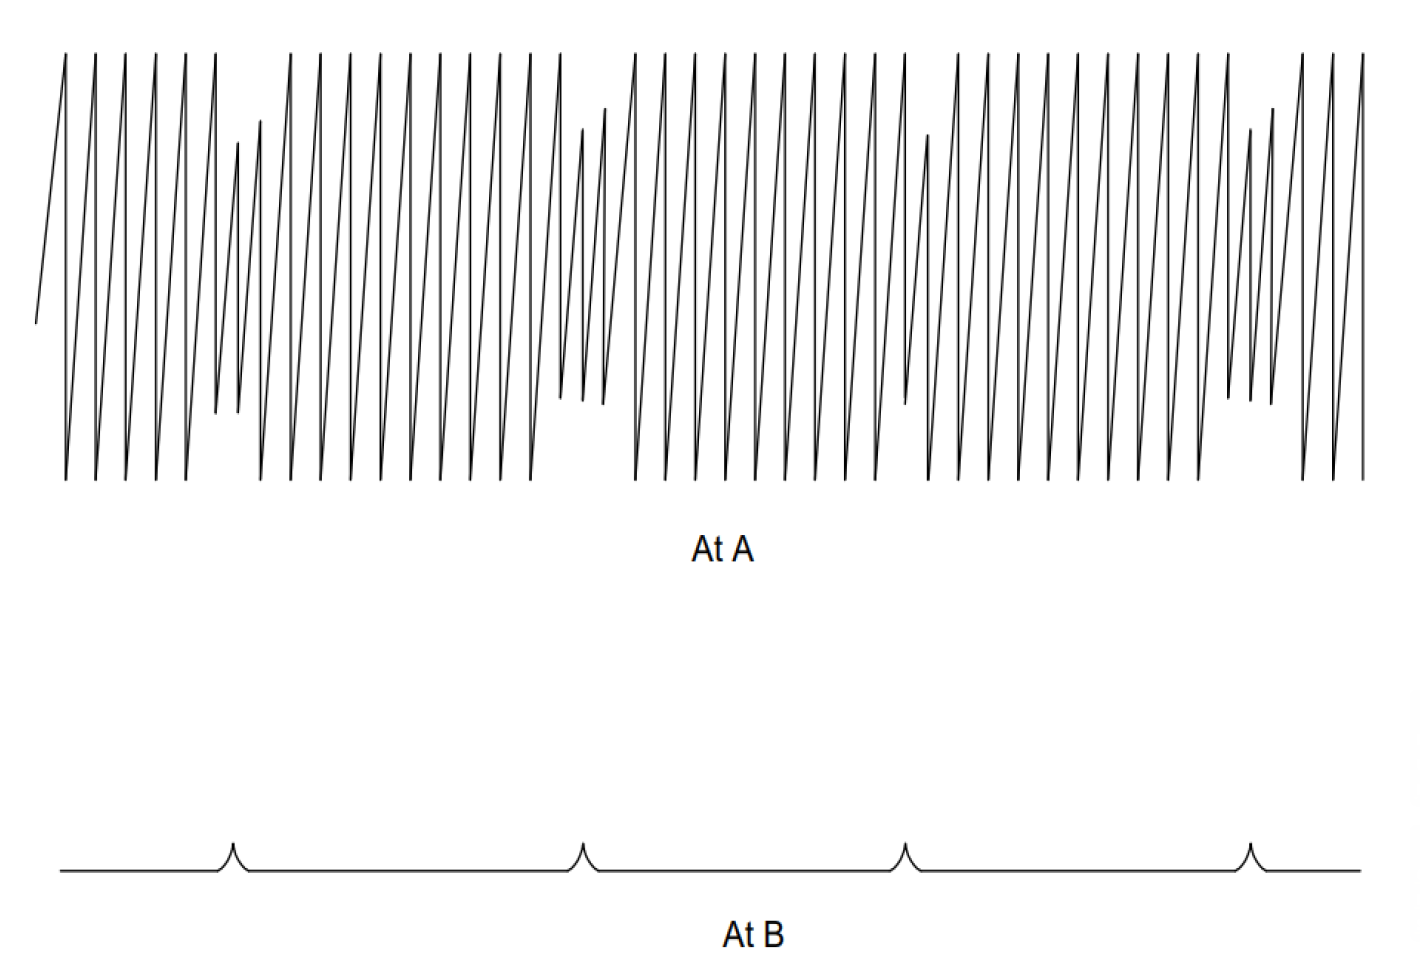
\includegraphics[width=0.5\textwidth]{peaks.png}
			\caption{\textbf{Occurence of Peaks}}
			\label{fig:4}
		\end{figure}

		Therefore g can be calculated by the following equation:

		$$g = \frac{h\nu_0}{\mu_0 H_0}$$

		here $h\;(=6.625\times 10^{-27} erg\;sec$) is the Plack's constant and $\mu_0\;(=0.927\times 10^{-20} erg/Gauss)$ is the permeability of free space.

		$$H_0 = H_{pp}\frac{Q}{P}$$

		Where $H_{pp}$ is the peak-to-peak value of the magnetic field, $Q$ is half the distance between the two peaks and $P$ is the maximum $X$ deflection. A magnetic field defined for RMS field H as:

		$$H_{pp} = 2\sqrt{2}H$$

		H, the RMS magnetic field between the Helmholtz coils is given by:

		$$H = \frac{32\pi nI}{10a\sqrt{125}}$$

		Putting appropriate values in the above equations, we get:

		\begin{equation}
			g = c\times \frac{\nu_0}{IQ} = 3.375\times 10^{-8} \times \frac{\nu_0}{m}
			\label{eq:1}
		\end{equation}

		where $c = \frac{5a\sqrt{125}}{32\pi n \sqrt{2}}\times\frac{Ph}{\mu_0} = 3.375\times 10^{-8}$ and $m$ is the slope of $Q$ vs $\frac{1}{I}$ graph.
